\section{Géopolitique de la ville de Québec}\label{sec:geopolitique_quebec}
Cette section va faire un historique rapide de la géopolitique de la ville de Québec. Ceci est principalement pour dégager des grandes époques où les frontières sont restées stables et illustrer la complexité de représenter les règlements de plusieurs juridictions. \par
On observe trois grandes raflées de fusions \parencite{ville_de_quebec_reperes_nodate}:
\begin{itemize}
  \item '65-'72:
  \SubItem{Duberger('70), Les Saules('70) et Neufchâtel ('71) rejoignent la ville de Québec}
  \SubItem{Ste-Foy et Ancienne Lorette fusionnent('70)}
  \SubItem{Le territoire de Wendake s'étend vers le Sud}
  \SubItem{Orsainville cède une péninsule de territoire à Charlesbourg}
  \SubItem{Beauport et Beauport-Ouest fusionnent('66)}
  \SubItem{Notre-Dame de Lorette devient L'Ancienne-Lorette('67)}
  \item '72-76:
  \SubItem{Charlesbourg, Orsainville, Charlesbourg-Est et Notre-Dame des Laurentides fusionnent pour devenir Charlesbourg ('76)}
  \SubItem{Charlesbourg-Ouest est annexé par Québec('76)}
  \SubItem{Giffard, Beauport, Courville, Villeneuve et Montmorency fusionnent('76) pour devenir Beauport}
  \SubItem{Val-Belair et Val-Saint-Michel fusionnent et deviennent Val-Belair('73)}
  \item '76-2001:
  \SubItem{Stabilité des limites territoriales}
  \item 2002:
  \SubItem{Fusion de Québec, L'Ancienne-Lorette, St-Augustin de Desmaures, Charlesbourg, Beauport, Val-Belair, Ste-Foy, St-Émile, Lac-St-Charles, Vanier, Cap-Rouge et Loretteville}
  \item 2006
    \SubItem{Séparation St-Augustin de Desmaures et L'Ancienne-Lorette}
\end{itemize}
\FloatBarrier
La figure \ref{fig:municipalites_carto_historique} montre l'évolution des barrières géopolitiques au cours du temps. 
\begin{figure}[ht]
  \centering
  \begin{subfigure}[t]{0.45\textwidth}
    \centering
    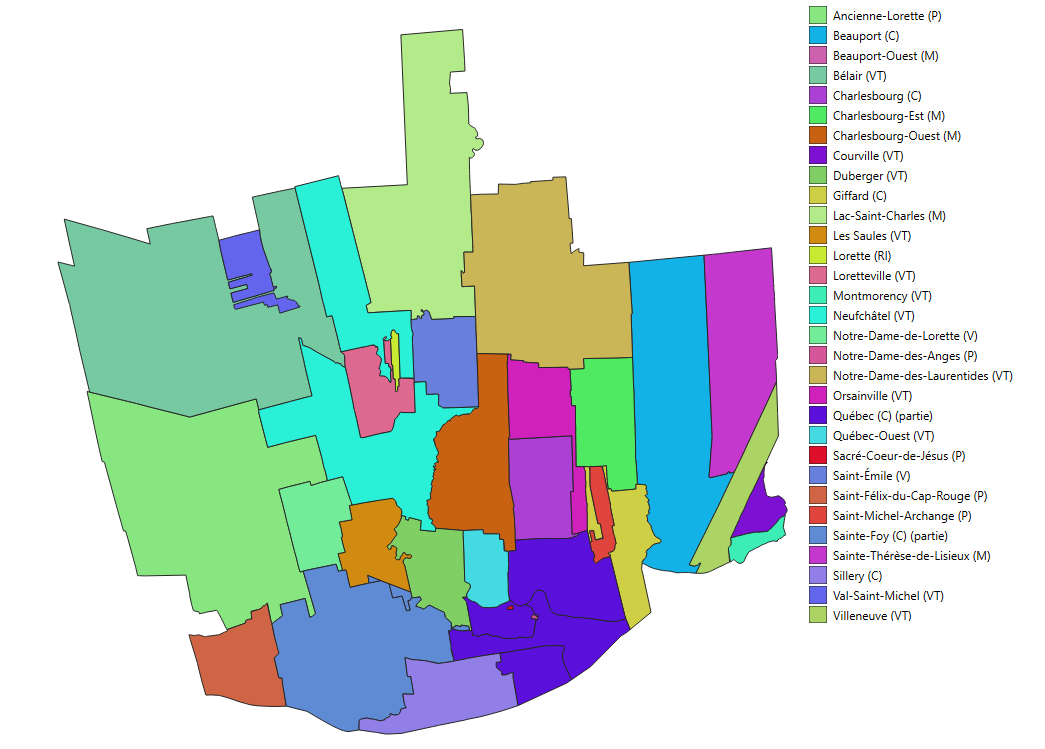
\includegraphics[width=0.9\linewidth]{images/municipalites_1965.png}
    \caption{1965}
    \label{fig:municipalites_1965}
  \end{subfigure}%
  \begin{subfigure}[t]{0.45\textwidth}
    \centering
    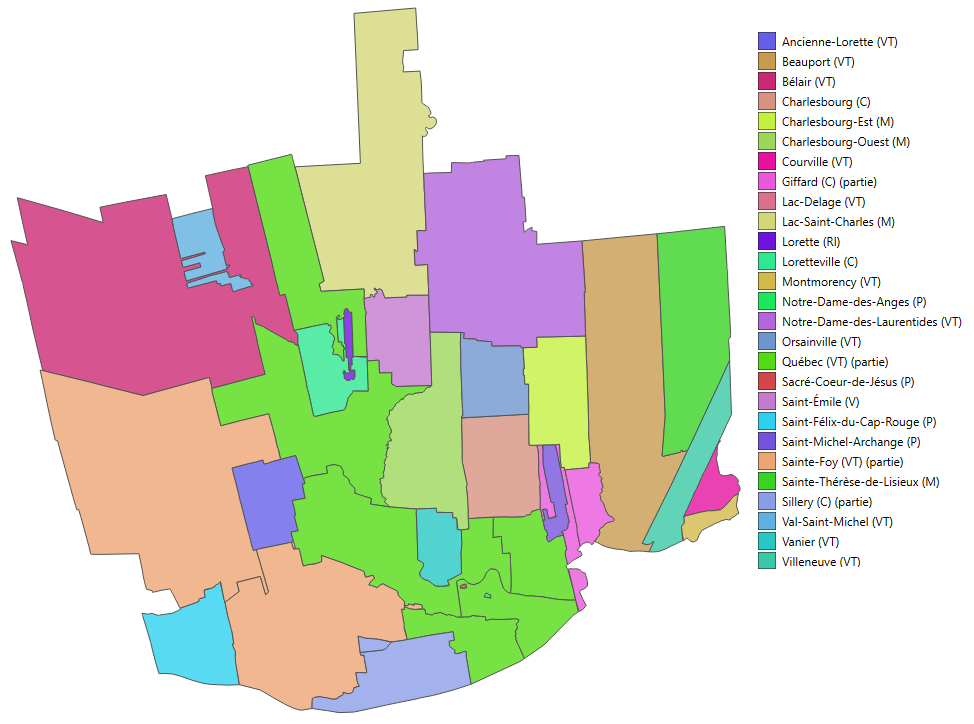
\includegraphics[width=0.9\linewidth]{images/municipalites_1972.png}
    \caption{1972}
    \label{fig:municipalites_1972}
  \end{subfigure}\\
  \begin{subfigure}[t]{0.45\textwidth}
    \centering
    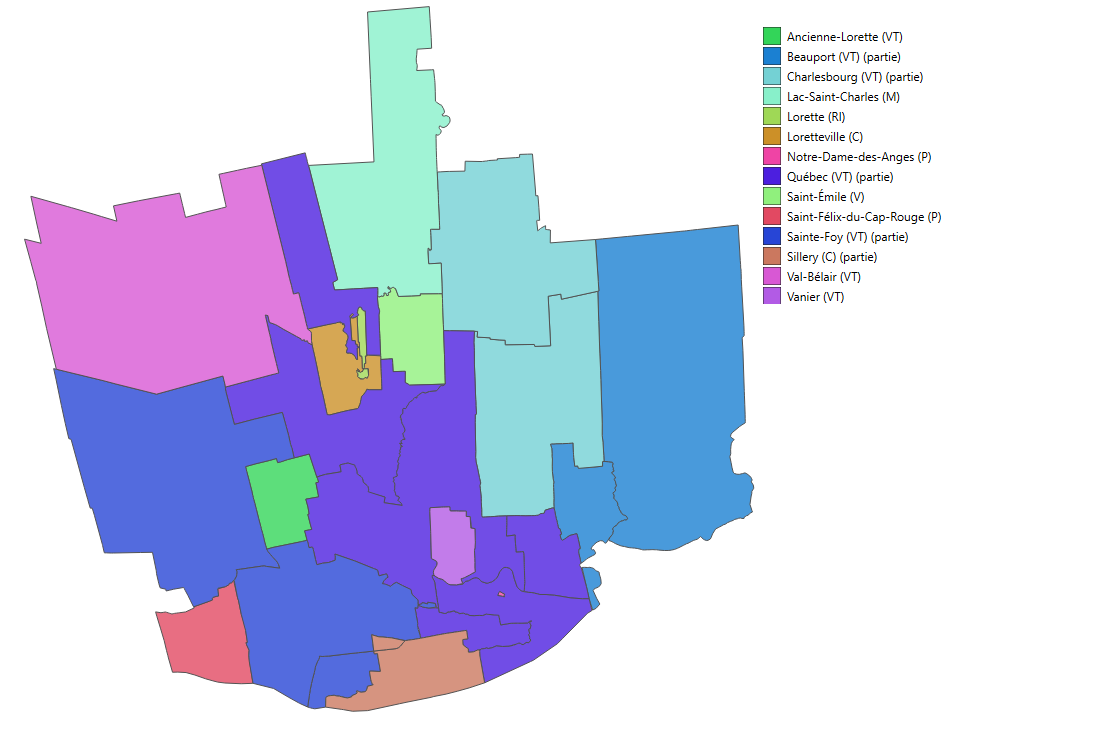
\includegraphics[width=0.9\linewidth]{images/municipalites_1980.png}
    \caption{1980}
    \label{fig:municipalites_1980}
  \end{subfigure}%
  \begin{subfigure}[t]{0.45\textwidth}
    \centering
    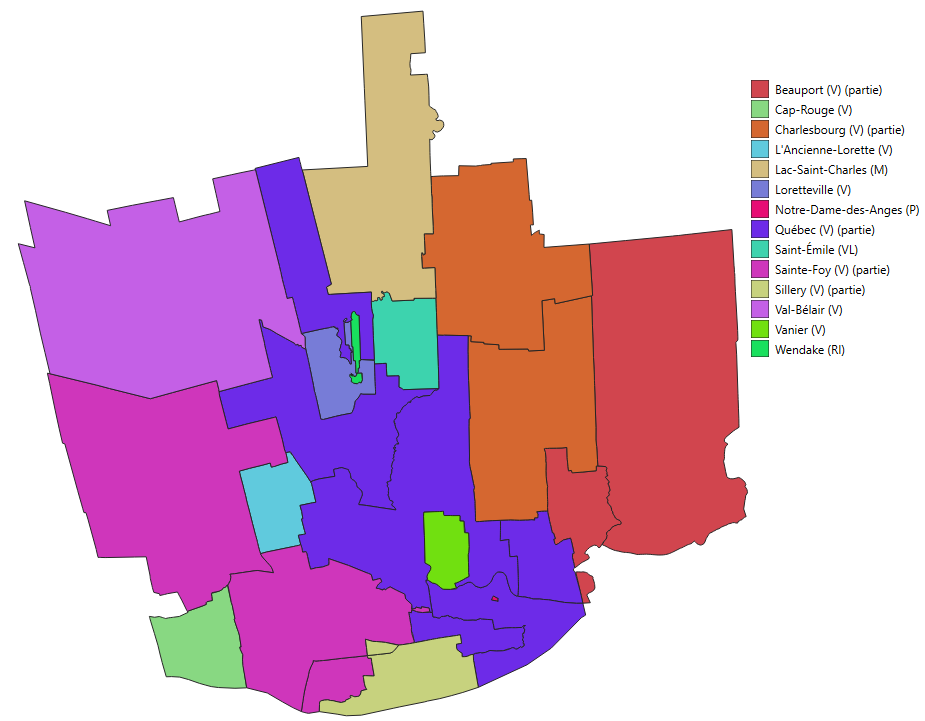
\includegraphics[width=0.9\linewidth]{images/municipalites_1988.png}
    \caption{1988}
    \label{fig:municipalites_1988}
  \end{subfigure}\\
  \begin{subfigure}[t]{0.45\textwidth}
    \centering
    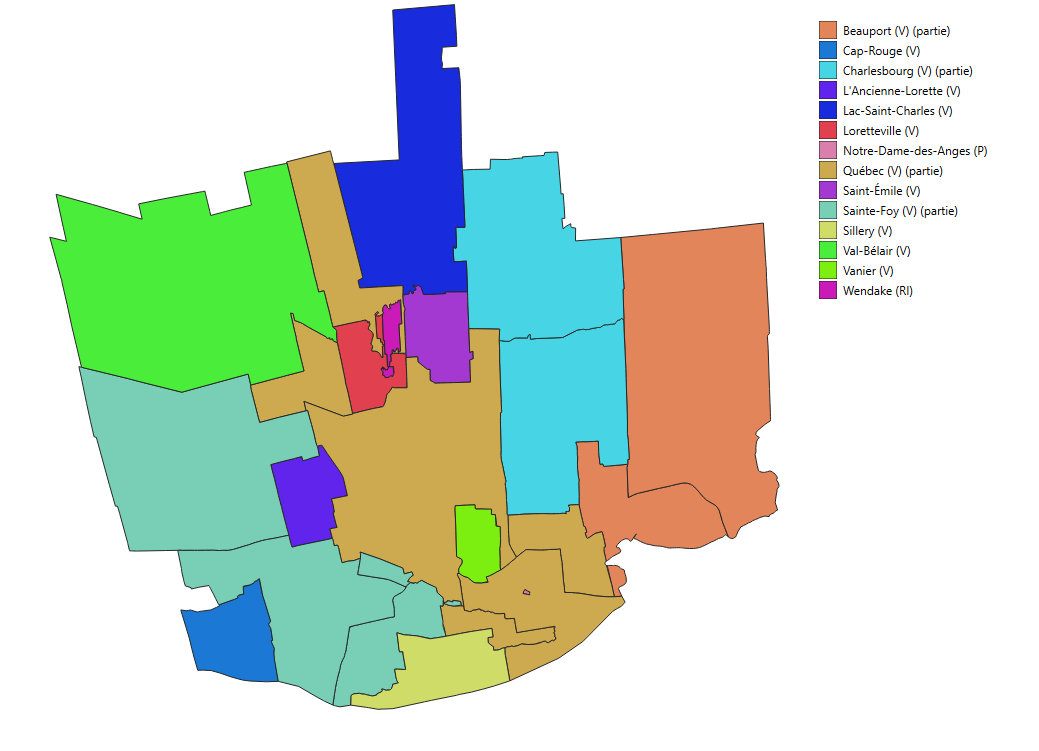
\includegraphics[width=0.9\linewidth]{images/municipalites_2001.png}
    \caption{2001}
    \label{fig:municipalites_2001}
  \end{subfigure}%
  \begin{subfigure}[t]{0.45\textwidth}
    \centering
    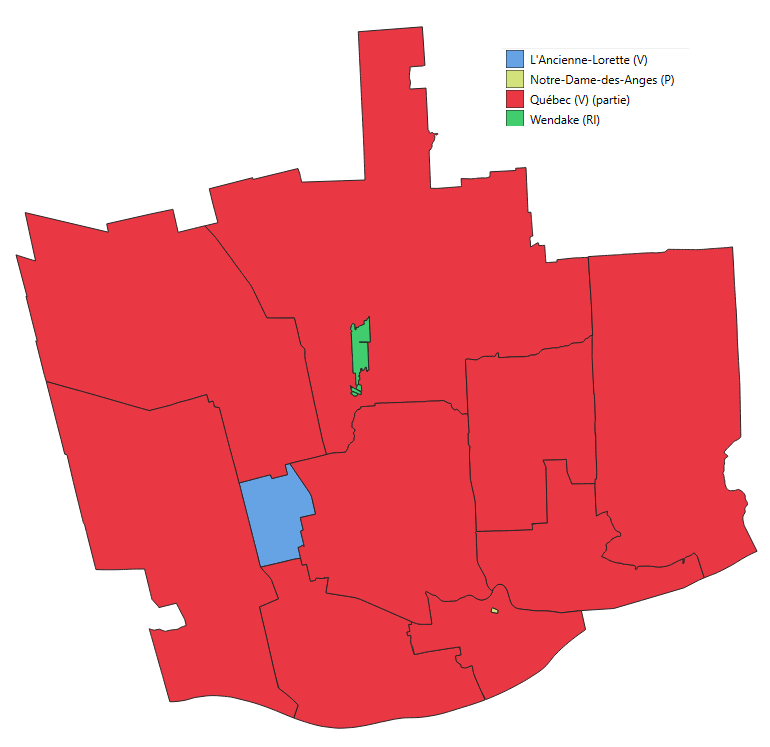
\includegraphics[width=0.8 \linewidth]{images/municipalites_2011.png}
    \caption{2011}
    \label{fig:municipalites_2011}
  \end{subfigure}%
  \caption{Séparation géopolitique du territoire de l'actuelle Ville de Québec \parencite{elections_quebec_atlas_2021}}\label{fig:municipalites_carto_historique}
\end{figure}

%Cela étant dit, l'historique de fusion de municipalités et la difficulté de trouver des codes d'urbanisme avant 1995 rend l'utilisation de ces données relativement difficile. La figure \ref{fig:historique_fusions} montre les fusions successives ayant mené à l'actuelle ville de Québec:
  %\begin{figure}[!h]
  %  \centering
  %  \captionsetup{justification=centering,margin=2cm}
  %  \includegraphics[width = 0.5\textwidth]{images/historique_fusions_VDQ.png}
  %  \captionsetup{justification=centering,margin=2cm}
  %  \caption{Diagramme montrant les fusions géopolitiques de la ville de Québec. \hl{Vérifier droits d'auteurs} Source: }
  %  \label{fig:historique_fusions}
  %\end{figure}
  %\FloatBarrier

%D'autre part, à travers les années '90, la ville de Québec va créer des requis de statinnement différents par quartiers. Post-fusion, les différentes villes garderont leurs codes d'urbanisme jusqu'en 2009 où la ville créera un code applicable à l'ensemble du territoire avec 4 sous zone: Général, Axe Structurant B, Axe Structurant A et Urbain Dense \parencite{VilledeQuebec:ReglementHarmonisation:2009}. La définition spatiale des unités de voisinage est donnée dans \textcite{VilledeQuebec:ZonageMunicipal:2024} et l'assignation de la zone est donnée dans \textcite{VilledeQuebec:GrilleSpecifications:2024}. La carte à la figure \ref{fig:types_unites_voisinage} montre les unités de voisinage pour la ville de Québec catégorisé selon la définition ci-haut:
\begin{figure}[ht]
  \centering
  \begin{subfigure}[t]{0.5\textwidth}
    \centering
    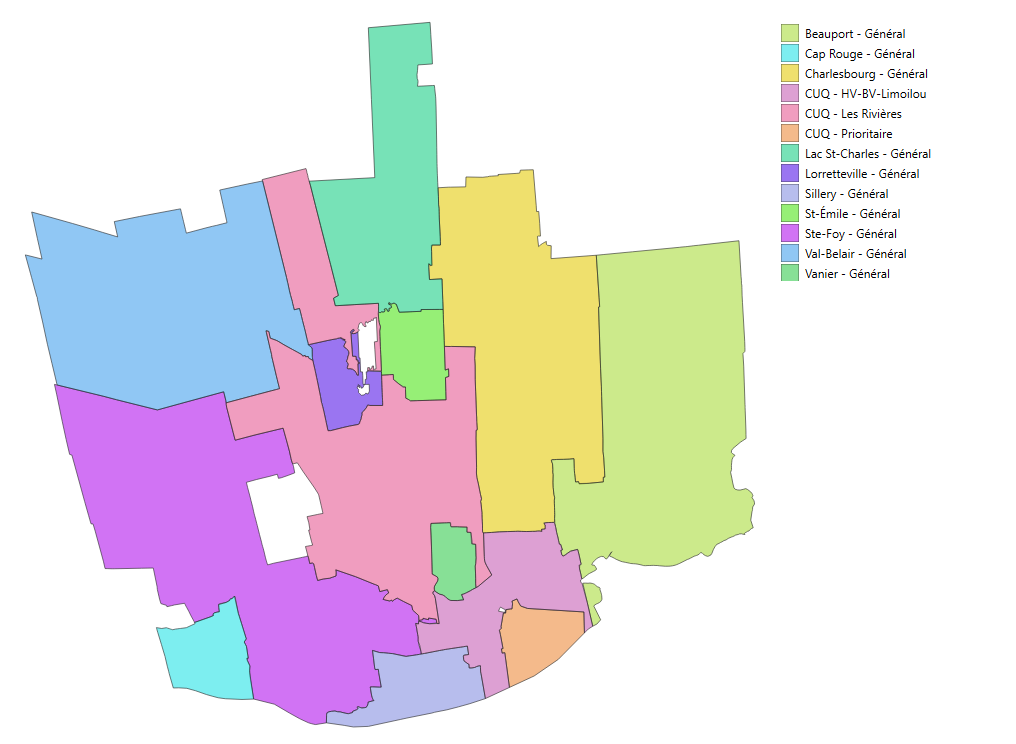
\includegraphics[width=0.9\linewidth]{images/geographie_code_urbanisme_1995-1997.png}
    \caption{1995-1997}
  \end{subfigure}~
  \begin{subfigure}[t]{0.5\textwidth}
    \centering
    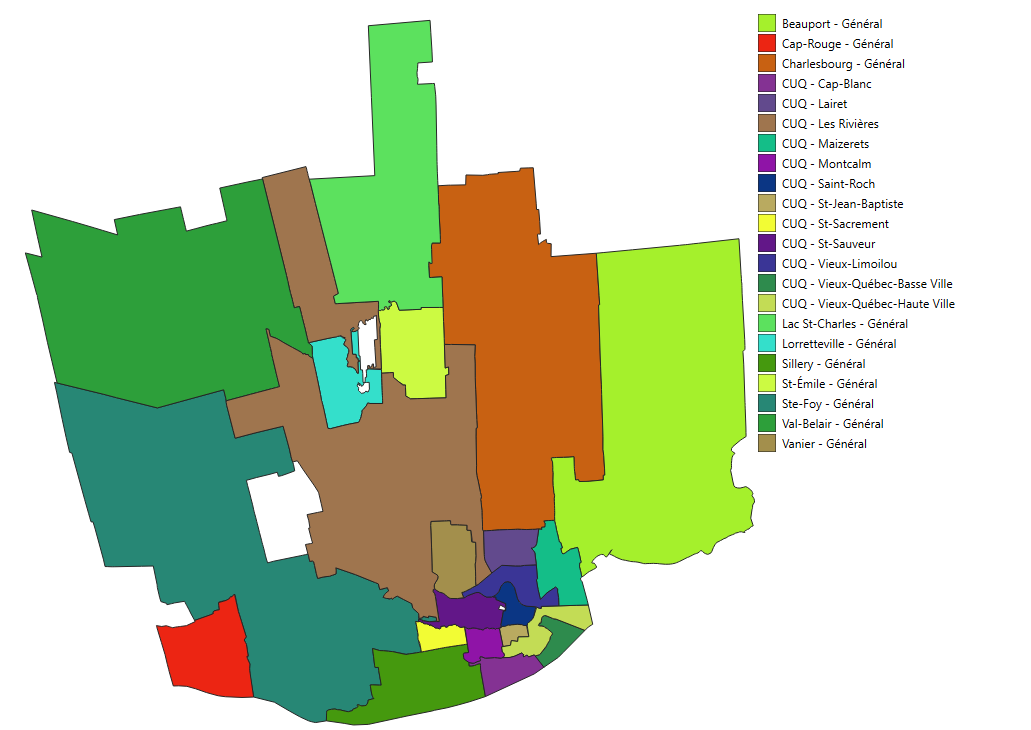
\includegraphics[width=0.9\linewidth]{images/geographie_code_urbanisme_1997-2009.png}
    \caption{1995-1997}
  \end{subfigure}\\
  \begin{subfigure}[t]{0.6\textwidth}
  \centering
  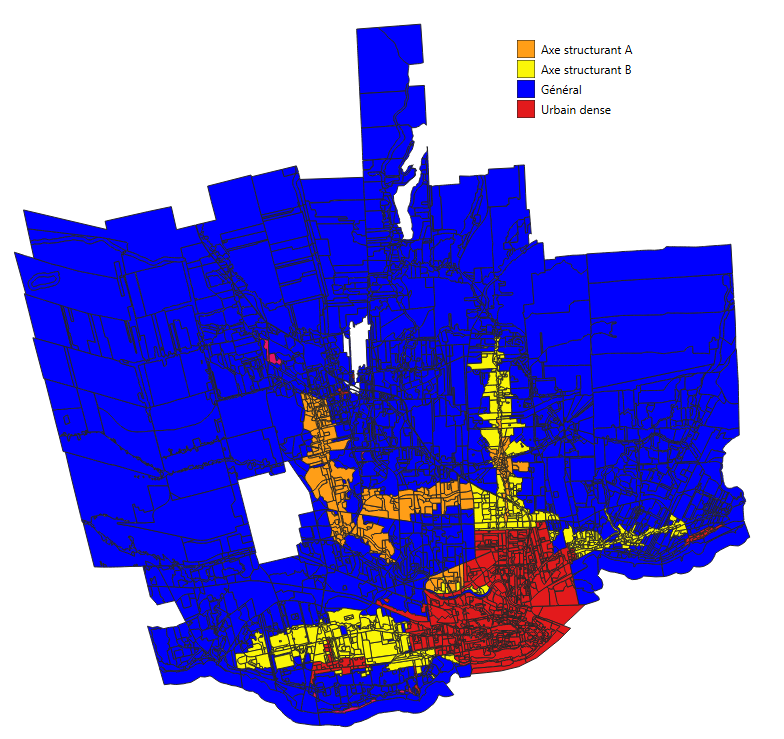
\includegraphics[width=0.8\linewidth]{images/geographie_code_urbanisme_2009_present.png}
  \caption{2010-présent}
  \end{subfigure}
  \caption{Secteurs ayant des minimum de stationnement différents}
  \label{fig:types_unites_voisinage}
\end{figure}
\FloatBarrier
\section{Politiques de stationnement de la ville de Québec} \label{sec:politiques_stationnement}

La ville de Québec est en processus d'abroger ces requis pour l'habitation pour les zones en milieu dense ou le long des axes de transport en commun \parencite{ville_de_quebec_adoption_2024}.\par
  En plus de l'hétérogénéité spatiale qui est décrite à la section \ref{sec:geopolitique_quebec}, on constate aussi une hétérogénéité au niveau des catégories utilisées pour les requis de stationnement. Ceci est d'autant plus ardu que les catégories utilisées dans les minimums de stationnement n'ont pas nécessairement d'équivalent direct dans le \ac{CUBF} utilisé dans le rôle foncier du Québec \parencite[Annexe 2C.1]{gouvernement_du_quebec_manuel_2024}. Le tableau \ref{tab:req_stat_presents} et la figure \ref{fig:n_utilisation_CUBF_minimums} résument la présence d'un requis de stationnement explicité ou inféré pour un code \ac{CUBF} donné \parencite{ville_de_quebec_adoption_2024,ville_de_quebec_reglement_1995}. Les codes d'urbanisme des municipalités pré-fusion sont issus d'un résumé fourni par la ville. Cette synthèse est nécessairement arbitraire: les catégories dans le code d'urbanisme ne sont pas constantes entre les codes avec différents niveaux de superposition ou catégorisation par municipalité, rendant une synthèse difficile. La synthèse est recalée sur les codes \ac{CUBF} pour la simple raison que cette donnée sera exploitée pour choisir la réglementation à appliquer pour inférer une capacité de stationnement requise. Les données sont issues d'une synthèse de la ville. Une demande a été complétée auprès du service de greffe pour obtenir les textes de loi.
  %\tiny
  \newcommand{\YCHECK}{\Checkmark}
  \newcommand{\NCHECK}{\cellcolor{red} \XSolid}
  \newcommand{\OCHECK}[1]{\cellcolor{orange} / #1}
  \newcolumntype{P}[1]{>{\centering\arraybackslash}p{#1}}
  \newcolumntype{M}[1]{>{\centering\arraybackslash}m{#1}}
  
  \setlength{\LTcapwidth}{\textwidth}
  \begin{landscape}
    \begin{center}
      \begin{longtable}{P{1.0cm} | p{7.5cm} | c || *{12}{P{5mm}}||p{6mm}} 
        \multirow{2}{*}{\STAB{\rotatebox[origin=c]{90}{Categ}}} & Juridiction & \STAB{\rotatebox[origin=c]{90}{Code \ac {CUBF}}} & \rotatebox[origin=c]{90}{  VDQ (2009-présent)} & \rotatebox[origin=c]{90}{VDQ (1995-2009)} & \rotatebox[origin=c]{90}{Beauport} & \rotatebox[origin=c]{90}{Cap-Rouge} & \rotatebox[origin=c]{90}{Charlesbourg} & \rotatebox[origin=c]{90}{Lac St-Charles} & \rotatebox[origin=c]{90}{Loretteville} & \rotatebox[origin=c]{90}{Sillery} & \rotatebox[origin=c]{90}{Ste-Foy} & \rotatebox[origin=c]{90}{St-Émile} & \rotatebox[origin=c]{90}{Val-Belair} & \rotatebox[origin=c]{90}{Vanier} & \rotatebox[origin=c]{90}{Nombre de requis} \\
        %& No. Règl. & MEFQ & R.V.Q. 1400 & V.Q.Z. 3 & 87-806 & 1151-95 & 96-2921 & 88-257 & 1386 & 950 & 3501 & 310-89 & VB-344-88 & 93-05-1245\\
        \hline  
        \endhead
        \hline
        \multicolumn{15}{c}{\Checkmark = Requis présent, \colorbox{red}{\XSolid} = Requis absent, \colorbox{orange}{/} = Requis implicite à une définition plus générale}\\\hline
        \endfoot
        \hline
        \multicolumn{15}{c}{\Checkmark = Requis présent, \colorbox{red}{\XSolid} = Requis absent, \colorbox{orange}{/} = Requis implicite à une définition plus générale}\\\hline
        \caption{Présence de règlementation de stationnement selon le code \ac{CUBF}}\label{tab:req_stat_presents}
        \endlastfoot
        \multirow{6}{*}{\STAB{\rotatebox[origin=c]{90}{Résidentiel}}} & Logement & 10XX & \YCHECK & \YCHECK &\YCHECK & \YCHECK &\YCHECK &\YCHECK& \YCHECK & \YCHECK & \YCHECK &\YCHECK & \YCHECK & \YCHECK&12\\
        & Logement subventionné & 10XX & \YCHECK & \YCHECK & \NCHECK & \NCHECK & \NCHECK& \NCHECK &\NCHECK &\NCHECK &\NCHECK &\NCHECK &\NCHECK & \NCHECK&2 \\
        & Habitation Collectives & 15XX & \YCHECK & \NCHECK & \YCHECK & \YCHECK & \YCHECK & \YCHECK & \YCHECK & \NCHECK & \NCHECK & \YCHECK & \YCHECK & \NCHECK&8 \\
        & Maison de chambres &  151X & \YCHECK & \YCHECK & \OCHECK{} & \OCHECK{} & \OCHECK{} & \OCHECK{} & \YCHECK & \NCHECK & \YCHECK &\OCHECK{} & \YCHECK & \YCHECK&6\\
        & Maison de retraite non autonomes & 1541 & \OCHECK{} & \YCHECK & \YCHECK & \YCHECK & \OCHECK{} & \OCHECK{} & \YCHECK & \YCHECK & \YCHECK & \OCHECK{} & \OCHECK{} & \NCHECK &6\\
        & Maison de retraite autonomes & 1543 & \OCHECK{} & \YCHECK & \YCHECK & \YCHECK & \OCHECK{} & \OCHECK{} & \YCHECK & \YCHECK & \YCHECK & \OCHECK{} & \OCHECK{} & \NCHECK&6 \\ 
        \hline
        \multirow{7}{*}{\STAB{\rotatebox[origin=c]{90}{Industriel / Infra.}}}& Industriel Général & \makecell[l]{2XXX\\3XXX} & \YCHECK & \YCHECK & \YCHECK & \YCHECK & \YCHECK & \YCHECK & \YCHECK & \YCHECK & \YCHECK & \YCHECK & \YCHECK & \YCHECK&12 \\
        & Industrie Haute Technologie & \makecell[l]{355X\\356X\\357X} & \YCHECK & \OCHECK{} & \OCHECK{}  & \OCHECK{}  & \OCHECK{}   & \OCHECK{}   & \OCHECK{}   & \OCHECK{}   &  \YCHECK & \OCHECK{}   & \OCHECK{}& \OCHECK{}&2 \\
        & Industrie mise en valeur et récupération &487X & \YCHECK & \OCHECK{} & \OCHECK{} & \OCHECK{} & \OCHECK{} & \OCHECK{} & \OCHECK{} & \OCHECK{} & \YCHECK & \OCHECK{} & \OCHECK{} & \OCHECK{}&2 \\ 
        & Entreposage & 637X & \YCHECK&\YCHECK&\OCHECK{}&\OCHECK{}&\OCHECK{}&\OCHECK{}&\YCHECK&\YCHECK&\OCHECK{}&\YCHECK&\YCHECK&\YCHECK &7\\
        & Service de construction & 66XX & \OCHECK{}  & \OCHECK{} &\OCHECK{} &\OCHECK{} &\OCHECK{} &\OCHECK{} & \YCHECK &\OCHECK{} &\OCHECK{} & \OCHECK{} & \OCHECK{} & \YCHECK&2\\
        \hline
        \multirow{4}{*}{\STAB{\rotatebox[origin=c]{90}{Commerces}}} & Centre et Immeuble Commercial & 50XX & \YCHECK & \YCHECK & \YCHECK & \YCHECK &\YCHECK&\YCHECK& \YCHECK&\YCHECK&\YCHECK&\YCHECK&\YCHECK&\YCHECK&12\\
        & Vente en gros & 51XX &\OCHECK{}&\YCHECK&\OCHECK{}&\OCHECK{}&\OCHECK{}&\OCHECK{}&\YCHECK&\OCHECK{}&\OCHECK{}&\OCHECK{}&\YCHECK&\OCHECK{}&3\\
        & Vente au détail construction et quincaillerie & 52XX&\OCHECK{}&\OCHECK{}&\OCHECK{}&\YCHECK&\OCHECK{}&\OCHECK{}&\YCHECK&\YCHECK&\YCHECK&\OCHECK{}&\YCHECK&\OCHECK{}&5 \\
        & Vente au détail marchandises & 53XX&\OCHECK{}&\OCHECK{}&\OCHECK{}&\OCHECK{}&\OCHECK{}&\OCHECK{}&\OCHECK{}&\OCHECK{}&\OCHECK{}&\OCHECK{}&\OCHECK{}&\OCHECK{}&0\\
        \multirow{6}{*}{\STAB{\rotatebox[origin=c]{90}{Commerces}}} & Vente au détail de l'alimentation & 54XX &\YCHECK&\YCHECK&\OCHECK{}&\OCHECK{}&\YCHECK&\YCHECK&\YCHECK&\YCHECK&\YCHECK&\YCHECK&\YCHECK&\YCHECK &10\\
        & Vente au détail de véhicules et produits connexes & 55XX &\YCHECK&\OCHECK{}&\OCHECK{}&\OCHECK{}&\OCHECK{}&\YCHECK&\YCHECK&\YCHECK&\YCHECK&\YCHECK&\YCHECK&\YCHECK&8\\
        & Station Essence & 553X&\YCHECK&\YCHECK&\YCHECK&\OCHECK{}&\OCHECK{}&\OCHECK{}&\YCHECK&\OCHECK{}&\YCHECK&\YCHECK&\YCHECK&\YCHECK&7 \\
        & Vente au détail de vêtements & 56XX&\OCHECK{}&\OCHECK{}&\OCHECK{}&\OCHECK{}&\OCHECK{}&\OCHECK{}&\YCHECK&\OCHECK{}&\YCHECK&\OCHECK{}&\OCHECK{}&\OCHECK{}&2\\
        & Vente au détail de mobilier & 57XX&\YCHECK&\YCHECK&\OCHECK{}&\OCHECK{}&\OCHECK{}&\OCHECK{}&\YCHECK&\OCHECK{}&\OCHECK{}&\OCHECK{}&\OCHECK{}&\OCHECK{}&3 \\
        & Vente au détail Autre & 59XX&\OCHECK{}&\OCHECK{}&\OCHECK{}&\OCHECK{}&\OCHECK{}&\OCHECK{}&\OCHECK{}&\OCHECK{}&\OCHECK{}&\OCHECK{}&\OCHECK{}&\OCHECK{}&0\\
        \hline
        \multirow{7}{*}{\STAB{\rotatebox[origin=c]{90}{Restaurants et bars}}} & Restaurant & 581X & \YCHECK&\NCHECK&\YCHECK&\NCHECK&\YCHECK&\YCHECK&\YCHECK&\YCHECK&\YCHECK &\YCHECK&\YCHECK&\YCHECK&7 \\
        & Restaurant plein service & \makecell{5811 \\ 5812 \\ 5815}& \OCHECK{}&\YCHECK&\OCHECK{}&\YCHECK&\OCHECK{}&\OCHECK{}&\OCHECK{}&\OCHECK{}&\OCHECK{}&\OCHECK{}&\OCHECK{}&\OCHECK{}&2\\
        & Restaurant service restreint/libre service& \makecell{5811 \\ 5812 }& \OCHECK{}&\YCHECK&\OCHECK{}&\YCHECK&\OCHECK{}&\OCHECK{}&\OCHECK{}&\OCHECK{}&\OCHECK{}&\OCHECK{}&\OCHECK{}&\OCHECK{}&2\\
        & Débit d'alcool & 582X&\YCHECK&\YCHECK&\YCHECK&\YCHECK&\YCHECK&\YCHECK&\YCHECK&\YCHECK&\YCHECK&\YCHECK&\YCHECK&\YCHECK&11\\
        \hline
        \multirow{3}{*}{\STAB{\rotatebox[origin=c]{90}{Tourisme}}} & Établissement d'hébergement & 583X&\YCHECK&\NCHECK&\NCHECK&\YCHECK&\YCHECK&\YCHECK&\YCHECK&\YCHECK&\YCHECK&\YCHECK&\YCHECK&\YCHECK&10\\
        & Hôtel & 5831&\OCHECK{}&\YCHECK&\YCHECK&\OCHECK{}&\OCHECK{}&\OCHECK{}&\OCHECK{}&\OCHECK{}&\OCHECK{}&\OCHECK{}&\OCHECK{}&\OCHECK{}&2\\
        & Môtel & 5832&\OCHECK{}&\YCHECK&\YCHECK&\OCHECK{}&\OCHECK{}&\OCHECK{}&\OCHECK{}&\OCHECK{}&\OCHECK{}&\OCHECK{}&\OCHECK{}&\OCHECK{}&2\\
        \hline
        & Services & 6XXX & \YCHECK & \YCHECK & \YCHECK &\YCHECK & \YCHECK & \YCHECK & \YCHECK & \YCHECK &\YCHECK &\NCHECK &\YCHECK&\NCHECK&10\\
        & Immeubles à bureaux & 60XX&\YCHECK&\YCHECK&\OCHECK{}&\YCHECK&\YCHECK&\YCHECK&\YCHECK&\YCHECK&\YCHECK&\NCHECK&\YCHECK&\NCHECK&9\\
        \multirow{19}{*}{\STAB{\rotatebox[origin=c]{90}{Services}}}& Finance, Assurance et Service immobilier & 61XX&\OCHECK{}&\YCHECK&\OCHECK{}&\OCHECK{}&\OCHECK{}&\OCHECK{}&\YCHECK&\OCHECK{}&\OCHECK{}&\YCHECK&\OCHECK{}&\YCHECK&4\\
        & Banque & 611X&\OCHECK{}&\YCHECK&\OCHECK{}&\YCHECK&\OCHECK{}&\YCHECK&\YCHECK&\YCHECK&\YCHECK&\OCHECK{}&\YCHECK&\OCHECK{}&7\\
        & Service personnels & 62XX & \OCHECK{} &\OCHECK{}&\OCHECK{}&\OCHECK{}&\YCHECK&\OCHECK{}& \OCHECK{}&\OCHECK{}&\YCHECK&\OCHECK{} &\OCHECK{}&\OCHECK{}&2\\
        & Salon de beauté / coiffure& 623X& \OCHECK{}&\YCHECK&\OCHECK{}&\OCHECK{}&\OCHECK{}&\OCHECK{}&\YCHECK&\OCHECK{}&\OCHECK{}&\OCHECK{}&\OCHECK{}&\YCHECK &3\\
        & Salon funéraire& 624X&\YCHECK&\YCHECK&\YCHECK&\YCHECK&\YCHECK&\YCHECK&\YCHECK&\YCHECK&\YCHECK&\YCHECK&\YCHECK&\YCHECK&12\\
        & Services d'affaires & 63XX &\OCHECK{}&\OCHECK{}&\YCHECK&\OCHECK{}&\OCHECK{}&\OCHECK{}&\YCHECK&\OCHECK{}&\OCHECK{}&\YCHECK&\OCHECK{}&\YCHECK&4\\
        & Services de réparation & 64XX&\OCHECK{}&\OCHECK{}&\OCHECK{}&\OCHECK{}&\OCHECK{}&\OCHECK{}&\OCHECK{}&\OCHECK{}&\OCHECK{}&\OCHECK{}&\OCHECK{}&\OCHECK{}&0\\
        & Service de réparation d'automobiles&641X&\YCHECK&\YCHECK&\YCHECK&\YCHECK&\OCHECK{}&\OCHECK{}&\YCHECK&\OCHECK{}&\YCHECK&\YCHECK&\YCHECK&\YCHECK&9\\
        & Service de réparation de mobiliers, d'équipements et de machines & 642X&\OCHECK{}&\OCHECK{}&\OCHECK{}&\OCHECK{}&\OCHECK{}&\OCHECK{}&\YCHECK&\OCHECK{}&\OCHECK{}&\OCHECK{}&\OCHECK{}&\OCHECK{}&1\\ 
        & Service de réparation de véhicules légers& 643X&\YCHECK&\YCHECK&\YCHECK&\YCHECK&\OCHECK{}&\OCHECK{}&\YCHECK&\OCHECK{}&\YCHECK&\YCHECK&\YCHECK&\YCHECK&9\\
        & Service de réparation et d'entretien de véhicules lourds& 644X&\YCHECK&\YCHECK&\YCHECK&\YCHECK&\OCHECK{}&\OCHECK{}&\YCHECK&\OCHECK{}&\YCHECK&\YCHECK&\YCHECK&\YCHECK&9\\
        & Service professionnel & 65XX&\YCHECK&\OCHECK{}&\YCHECK&\YCHECK&\OCHECK{}&\OCHECK{}&\OCHECK{}&\OCHECK{}&\OCHECK{}&\OCHECK{}&\OCHECK{}&\OCHECK{}&0\\
        & Service médical et de santé & 651X&\YCHECK&\YCHECK&\OCHECK{}&\OCHECK{}&\YCHECK&\YCHECK&\YCHECK&\YCHECK &\YCHECK & \OCHECK{} &\YCHECK & \OCHECK{}&9\\
        & Service d'hôpital & 6513 &\YCHECK &\YCHECK &\YCHECK &\YCHECK&\YCHECK&\YCHECK&\YCHECK&\YCHECK&\YCHECK&\YCHECK&\YCHECK&\YCHECK&12\\
        & Sanatorium, maison de convalescence et de repos & 6516 &\YCHECK &\YCHECK &\YCHECK&\OCHECK{}&\YCHECK &\YCHECK&\YCHECK&\YCHECK&\YCHECK&\YCHECK&\YCHECK&\YCHECK&11\\
        \multirow{12}{*}{\STAB{\rotatebox[origin=c]{90}{Services}}}& Service gouvernemental&67XX&\OCHECK{} & \OCHECK{} &\OCHECK{}&\OCHECK{}&\OCHECK{} &\OCHECK{} & \YCHECK&\OCHECK{}&\YCHECK&\YCHECK&\YCHECK&\YCHECK &5 \\
        & Pompiers/Police &672X&\YCHECK & \YCHECK &\OCHECK{}&\OCHECK{} &\OCHECK{} & \OCHECK{}&\OCHECK{}&\YCHECK&\OCHECK{}&\YCHECK&\OCHECK{}&\OCHECK{}&4\\
        & Service éducationnel&68XX&\YCHECK&\YCHECK&\NCHECK&\YCHECK&\NCHECK&\YCHECK&\YCHECK&\YCHECK&\NCHECK&\YCHECK{}&\YCHECK&\YCHECK &9 \\
        & Service de garderie&6541&\YCHECK&\OCHECK{}&\OCHECK{}&\OCHECK{}& \YCHECK&\OCHECK{}& \YCHECK &\OCHECK{}&\YCHECK&\OCHECK{}&\YCHECK&\OCHECK{}&5 \\
        & École Maternelle&6811&\OCHECK{}&\OCHECK{}&\OCHECK{}&\OCHECK{}&\OCHECK{}&\OCHECK{}&\YCHECK&\OCHECK{}&\YCHECK&\OCHECK{}&\YCHECK{}&\YCHECK{}&4 \\
        & École Primaire&6812&\YCHECK&\YCHECK&\YCHECK&\YCHECK&\YCHECK&\YCHECK&\YCHECK&\YCHECK&\YCHECK&\OCHECK{}&\YCHECK&\YCHECK&11 \\
        & École Secondaire / Polyvalente&\makecell{6813\\6822}&\YCHECK&\YCHECK&\YCHECK&\OCHECK{}&\YCHECK& \YCHECK&\YCHECK&\YCHECK&\YCHECK&\OCHECK{}&\YCHECK&\YCHECK&10 \\
        & CÉGEP &6823&\YCHECK&\YCHECK&\YCHECK&\OCHECK{}&\OCHECK{}&\YCHECK&\YCHECK&\OCHECK{}&\YCHECK&\OCHECK{}&\OCHECK{}&\OCHECK{}&6\\
        & Université&6821&\YCHECK&\YCHECK&\YCHECK&\OCHECK{}&\YCHECK&\YCHECK&\YCHECK&\OCHECK{}&\YCHECK&\OCHECK{}&\OCHECK{}&\OCHECK{}&7\\ 
        & Services religieux &691X&\YCHECK&\OCHECK{}&\YCHECK&\YCHECK&\OCHECK{}&\YCHECK&\YCHECK&\YCHECK&\YCHECK&\OCHECK{}&\YCHECK&\YCHECK&9\\
        \hline
        \multirow{8}{*}{\STAB{\rotatebox[origin=c]{90}{Culture et Récréation}}} & Culture, Récréation et Loisirs&7XXX &\NCHECK&\YCHECK&\YCHECK&\NCHECK&\YCHECK&\YCHECK&\NCHECK&\YCHECK&\NCHECK&\YCHECK&\YCHECK&\YCHECK&8\\
        & Activité Culturelle(Musée, Biblio) &711X&\YCHECK&\YCHECK&\YCHECK&\YCHECK&\YCHECK&\YCHECK&\YCHECK&\YCHECK&\YCHECK &\OCHECK{} &\OCHECK{} &\OCHECK{}&9\\
        & Assemblée de loisirs(Théâtre, Cinéma) &721X&\YCHECK&\YCHECK&\YCHECK& \YCHECK& \YCHECK&\YCHECK&\YCHECK&\YCHECK&\YCHECK&\OCHECK{}&\YCHECK&\OCHECK{}&10 \\
        & Installation sportive (Stade, Hippodrome)&722X&\YCHECK&\OCHECK{}&\OCHECK{}&\NCHECK&\OCHECK{}&\OCHECK{}&\YCHECK&\OCHECK{}&\YCHECK&\OCHECK{}&\OCHECK{}&\OCHECK{}&3\\
        & Centre de congrès&723X& \OCHECK{} & \YCHECK & \OCHECK{} & \NCHECK & \OCHECK{} & \OCHECK{}& \YCHECK& \OCHECK{} & \OCHECK{} & \OCHECK{} & \OCHECK{} & \OCHECK{}&2 \\
        & Activités récréatives&74XX&\YCHECK&\OCHECK{}&\YCHECK&\NCHECK&\OCHECK{}&\OCHECK{}&\YCHECK&\OCHECK{}&\YCHECK&\OCHECK{}&\OCHECK{}&\OCHECK{} &4\\
        & Terrains de golf&\makecell{7411\\7412}& \YCHECK& \OCHECK{}&\OCHECK{}&\NCHECK&\OCHECK{}&\OCHECK{}&\YCHECK&\OCHECK{}&\YCHECK&\YCHECK&\OCHECK{}&\OCHECK{}&4\\
        & Arena& 7451& \YCHECK&\YCHECK&\OCHECK{}&\NCHECK&\OCHECK{}&\OCHECK{}&\YCHECK{}&\YCHECK&\OCHECK{}&\YCHECK&\YCHECK&\OCHECK{}&6\\
        & Parcs/Camps &\makecell{75XX\\76XX}&\YCHECK &\NCHECK&\NCHECK&\NCHECK&\NCHECK&\NCHECK&\NCHECK&\NCHECK&\YCHECK&\YCHECK&\NCHECK&\YCHECK&5 \\
        \hline
        N/A & Extraction de ressources / Agriculture & 8XXX&\YCHECK&\NCHECK&\NCHECK&\NCHECK&\NCHECK&\NCHECK&\YCHECK&\NCHECK&\YCHECK&\NCHECK&\NCHECK&\NCHECK&3\\
      \end{longtable}
    \end{center}  
    \begin{figure}[h]
      \centering
      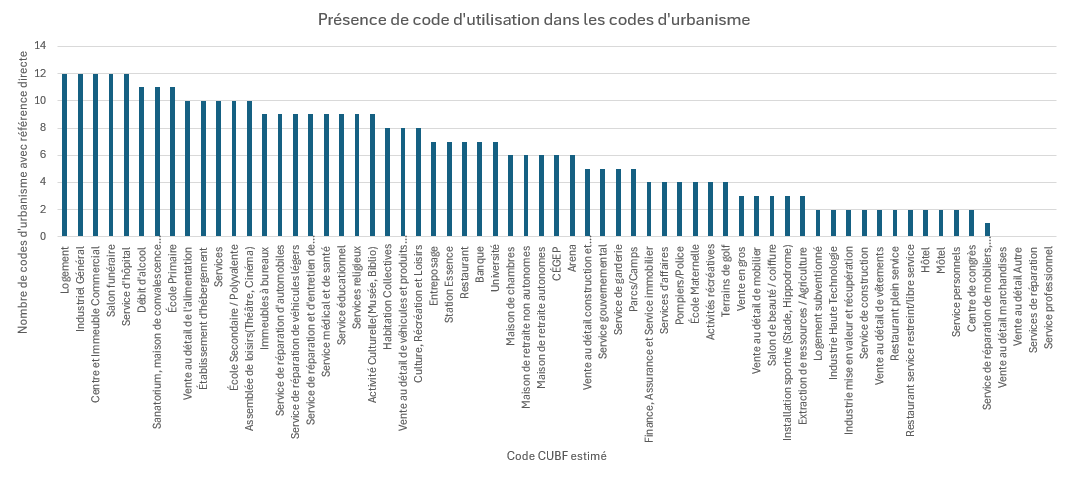
\includegraphics[width=22cm]{images/presence_requis_par_CUBF}
      \caption{Nombre de codes d'urbanisme utilisant les codes d'utilisation listés}\label{fig:n_utilisation_CUBF_minimums}
    \end{figure}
  \end{landscape}
  %\normalsize
  \FloatBarrier
  
  Les objets sur lesquels sont basés les codes d'urbanisme sont aussi hétérogènes. Bien que la plupart des requis soient basé sur une surface de plancher, certains sont exprimés en fonction d'autres objets considérés pertinents. D'autre part, la même utilisation du sol n'est pas nécessairement légiférée en utilisant le même objet entre deux juridictions différentes. Le tableau \ref{tab:objet_pour_inference_capacite} synthétise les objets considérés et les usages pour lesquels ils sont utilisés.

  \begin{table}[h]
    \centering
    \begin{tabular}{p{4cm} p{8cm}}
      \hline
      Objets considéré & Usages pertinents \\
      \hline
      Superficie de plancher & Majoritaire\\
      Superficie par usage (bureau, plateau TV) & Station télé \\
      Superficie de terrain & parc, zoo \\
      Logement & Logement \\
      Chambres & Maison de chambres, hébergement touristique, établissement de santé\\
      Lit & Établissement de santé, auberges de jeunesse, établissement carcéral \\
      Baie de service & Commerces liés à l'automobile\\
      Siège & Lieux de rassemblement, cinéma, théâtres, stades \\
      Salle & Cabinet médical, établissement scolaire, salon funéraire\\
      Personne & Débit d'alcool\\
      Employé & Services et vente au détail\\
      Médecin & Établissement de santé\\
      Étudiant & Établissement scolaire\\
      Plateau sportif & Golf, tennis, quilles, billards\\
      Poste de travail & Services personnels (salon de beauté)\\
      \hline
    \end{tabular}
    \caption{Récapitulatif des objets considérés pour fixer les capacité de stationnement}\label{tab:objet_pour_inference_capacite}
  \end{table}
  

  \FloatBarrier